\documentclass[acmtog]{acmart}
\usepackage{graphicx}
\usepackage{subfigure}
\usepackage{natbib}
\usepackage{listings}
\usepackage{bm}
\usepackage{amsmath}

\definecolor{blve}{rgb}{0.3372549 , 0.61176471, 0.83921569}
\definecolor{gr33n}{rgb}{0.29019608, 0.7372549, 0.64705882}
\makeatletter
\lst@InstallKeywords k{class}{classstyle}\slshape{classstyle}{}ld
\makeatother
\lstset{ %
backgroundcolor=\color{white},   % choose the background color
basicstyle=\footnotesize\ttfamily,        % size of fonts used for the code
columns=fullflexible,
breaklines=true,                 % automatic line breaking only at whitespace
captionpos=b,                    % sets the caption-position to bottom
tabsize=4,
commentstyle=\color{mygreen},    % comment style
escapeinside={\%*}{*)},          % if you want to add LaTeX within your code
keywordstyle=\color{blue},       % keyword style
stringstyle=\color{mymauve}\ttfamily,     % string literal style
frame=single,
rulesepcolor=\color{red!20!green!20!blue!20},
% identifierstyle=\color{red},
language=c++,
}
\lstset{basicstyle=\ttfamily}

% Title portion
\title{Final project:\\ {Photon mapping}} 

\author{Name:\quad Group19  \\ student number:\ 2020533010, 2020533013, 2020533042
\\email:\quad sunwl1@shanghaitech.edu.cn}

% Document starts
\begin{document}
\maketitle

\vspace*{2 ex}

\section{Introduction} 

\quad This is the final project of class CS171.01 class: Computer graphics, an implementation on photon mapping. 
In this part of the project report, we will briefly explain the implementation we have taken on this project
and also show the output result of photon mapping. We learn PM, PPM, SPPM step by step, finaly, we choose the method of Stochastic progressive photon mapping
as our main algorithm to implement this project.

Our job mainly contains Stochastic progressive photon mapping, KD tree and some rendering. 

\section{Implementation Details}

\quad \textbf{Part 1: Paper reading}

Before we introduce the paper on the Stochastic progressive photon mapping, we will firstly introduce what the photon mapping is. Photon mapping can get a higher efficiency at the cost of some space and time.

Photon mapping is an algorithm of two-pass. The first pass is photon tracing and the second pass is rendering(ray tracing). The first photon tracing pass is that photons which carry energy are emitted from the light source image scene, and then interact with the object surface in the scene whether reflection or refraction, and are recorded at the intersection of objects with a non-shiny surface. Finally, these photons are stored in a global photon map.

However, the efficiency of space and time is low. Then PPM comes. So what is progressive photon mapping? In the first step, the eye sample is organized into a kd tree structure, then photons are emitted round by round. r is reduced once in each round and a picture is rendered in each round. With the increase of the number of rounds, the number of photons become more and more while the value of r is becoming smaller and smaller,leading to the better result.

Then comes to the Stochastic progressive photon mapping, it is a slight improvement of ppm algorithm. Different from ppm, the stochastic progressive photon mapping is re-performed after each round of photon emission. In addition, each eye tracing will bring a random disturbance, so that the data in the eye sample kd-tree constructed each time are different.

The relation between PM, PPM, SPPM is shown clearly in the picture below.
In our implemention, we choose SPPM. It is a multi-pass algorithm meaning that the first pass is ray tracing and the other passes are photon tracing. More detailed implementation will be explained in the report after.
\begin{figure}[h]
	\centering
	{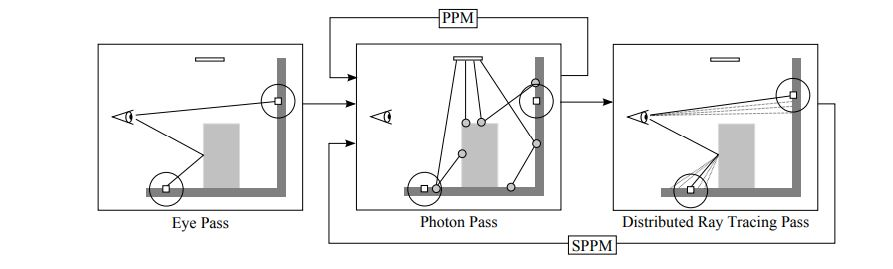
\includegraphics[width=8cm]{SPPM.JPG}}
\end{figure}

\quad \textbf{Part 2: Stochastic progressive photon mapping}

The ray tracing and the photon tracing are similar. We write the process of tracing in the same function. And we pass different parameters to the function to simulate the 2 different tracing.

In this tracing function, we use the trick: Russian Roulette. When the surfaces of specular are too many, the length of the tracing can be limited by Russian Roulette algorithm.

\quad \textbf{Russian Roulette}

It is a random algorithm to limit the length of tracing. It means that if we only sum all the tracing together then its efficiency will be low. In this time we can use Russian roulette algorithm to randomly skip some of the functions with low weight according to a specific rule, then we can get a higher efficiency. \\
% \begin{lstlisting}
%     double s = brdf_settings[next_face->BRDF].specular + brdf_settings[next_face->BRDF].diffuse + brdf_settings[next_face->BRDF].refraction;
%     double action = Utils::my_random(0,1) * s;
% \end{lstlisting}


In our tracing function, we divide the whole code into three parts: specular, diffuse and refraction. In the specular part, we only need to continue the ray tracing to next face which will be interacted with. Then the action initialized in the Russian Roulette algorithm will minus its specular, so that it can limit the ray tracing.

In the diffuse part, in the ray tracing pass, after Russian Roulette, we record the information of hitpoint: update the flux light and the weight, and if it hits light, we update the flux light and set the valid to false, otherwise we only set the valid to true. In the diffuse part, in the photon tracing pass, we need to update the hitpoint kd-tree(the detailed information will be discussed in Part3).

In the refraction part, we define a theta in and theta out to calculate the refraction. It is similar to our CG HW4's bonus. If it is a total reflection, then we only need to recursively do the next pass, otherwise we use schlick's approximation to calculate a Fresnel factor and consider both the reflection and the refraction. Then we recursively do the tracing.

After completing the tracing function in scene.cpp, we begin our SPPM algorithm. This part is implemented in the render function in the camera.cpp. 

As the explanation in part 1, the first pass is ray tracing. 
It is another form that can be described as a photon tracing from the camera. 
The ray will be reflected when it meet with specular and last until it is absorbed in the diffuse face. And we record the information of the hitpoint.

The next pass is photon tracing, the photons start from the light and we do the tracing, update the information of the hitpoint.

After the 2 passes, we evalute the radiance use the formula below.
\begin{figure}[h]
	\centering
	{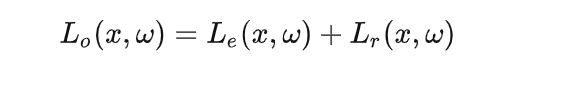
\includegraphics[width=8cm]{l.JPG}}	
\end{figure}
\begin{figure}[h]
	\centering
	{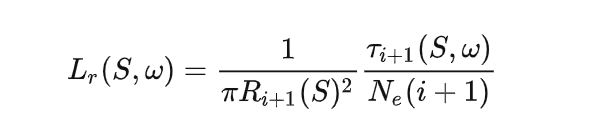
\includegraphics[width=8cm]{lr.JPG}}	
\end{figure}



\quad \textbf{Part 3: kd-tree construction}
\begin{figure}[h]
	\centering
	{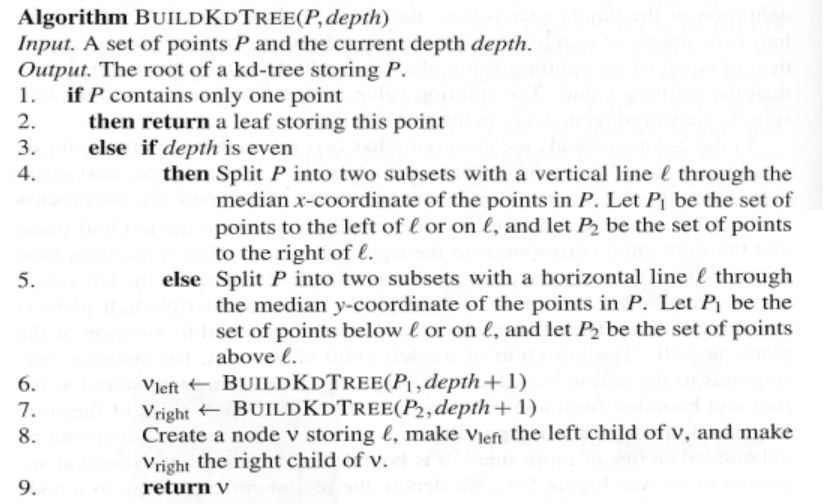
\includegraphics[width=8cm]{kdtree.JPG}}	
	\caption{2D case}
\end{figure}

To speed up photon mapping, a positionally balanced kd-tree needs to be constructed for the photon graph.
The picture above is the peseudo code we learn from the internet. It shows how to build a kd-tree in a 2D case.
As for this project, we need to build a kd-tree with 3 dimension similarly. This part is written in the hitpoint.cpp.
If the dimension is 0, we compare the eigen vector's first element and get the median in this axis, which means if defining a vector3f a, we compare the x of a and get the median. Similarly, if the dimension is 1, we compare the y and get the median, if the dimension is 2, we compare the z and get the median. 
After the previous steps, we build the left child tree and the right child tree of the node recursively.

The update of the kd-tree is more important. It is actually the core part of the SPPM. We need to update the information during the passes.
The fomula of the updating is shown below. 
% \begin{figure}[h]
% 	\centering
% 	{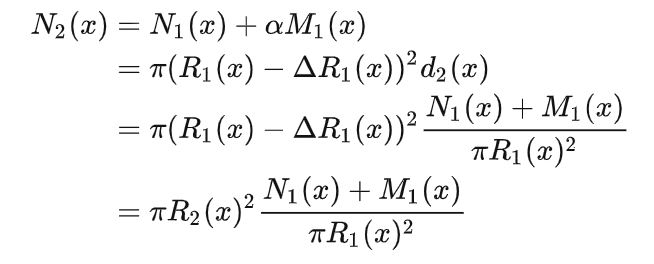
\includegraphics[width=8cm]{n.JPG}}	
% \end{figure}
\begin{figure}[h]
	\centering
	{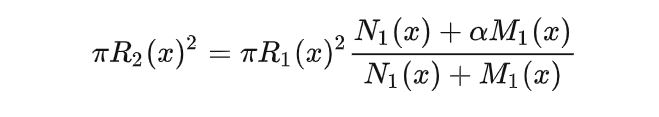
\includegraphics[width=8cm]{r.JPG}}	
\end{figure}
\begin{figure}[h]
	\centering
	{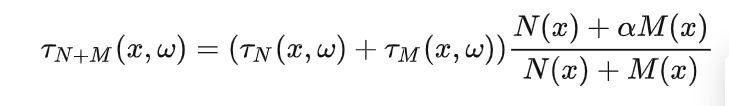
\includegraphics[width=8cm]{t.JPG}}	
\end{figure}
% \begin{figure}[h]
% 	\centering
% 	{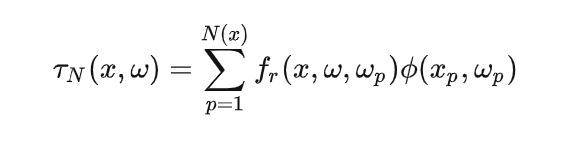
\includegraphics[width=8cm]{tn.JPG}}	
% \end{figure}

The above steps is to construct a hitpoint kd-tree. Besides, we also construct an object kd-tree to improve efficiency. 
This part is implemented in the scene.cpp.

\quad \textbf{Part 4: Details}
The random double number generating tool (in src/utils.cpp) we use is mt19937 from c++11, along with ctime. A double random is often used by Russion Roulette, but sometimes needed by genertating or sampling rays, in which case we use apply a Quasi-Monte Carlo method to it, with halton sequence.
\section{result}
\begin{figure}[h]
	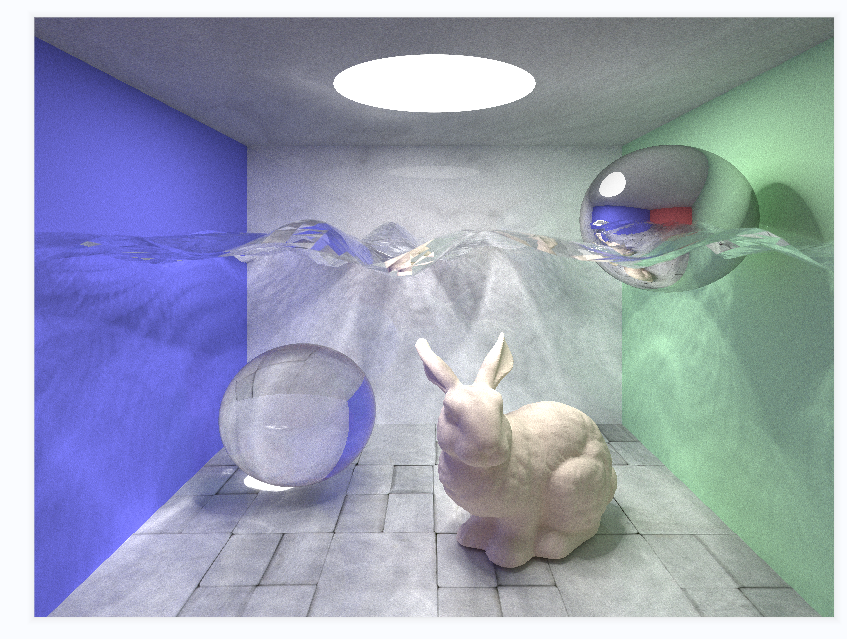
\includegraphics[width=8cm,height=6cm]{result.png}
	\caption{result}
\end{figure}
Fig.2 is the final result of out project, the resolution is 800*600, the loop round number is 600 and the number of photon is 200000.
\begin{figure}[h]
	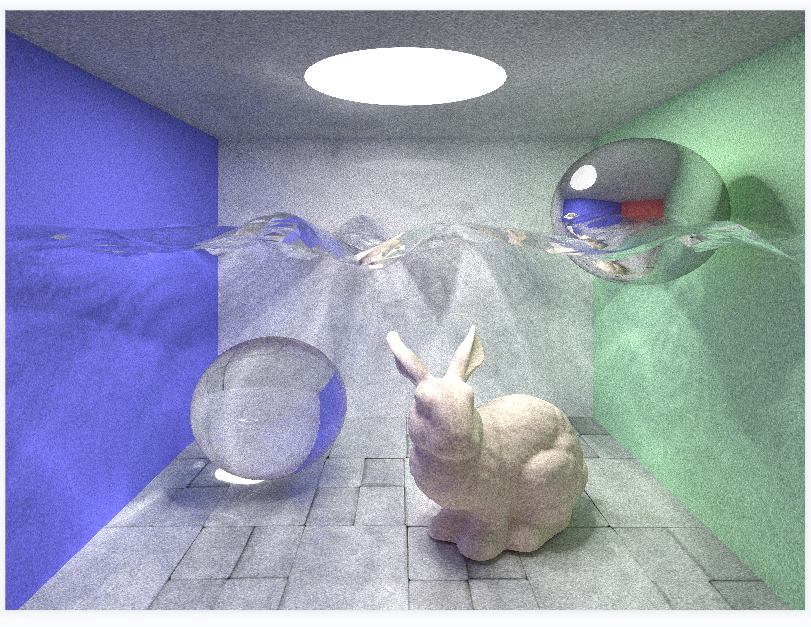
\includegraphics[width=8cm,height=6cm]{result100.png}
	\caption{result with weaker para}
\end{figure}

Fig.3 is the result with weaker parameter, 100 rounds and still 200000 photons. It surely looks dimmer and rougher than the final one.

The result contains a glass sphere, and mirror sphere, a textured bottom, marble walls, a disc light and a bunny.


\section{Work distribution} 

Our group's work distribution is almost equal. And we read the paper, learn the SPPM, do the most coding, debugging together by tencent meeting.
The detailed work distribution is shown below.

Sun Weiliang (2020533010): The whole frame, object.cpp, texture.cpp

Tian Haoyuan (2020533013): scene.cpp(tracing fucntion), camera.cpp(SPPM)

Fan gucongcong (2020533042): hitpoint.cpp(kdtree), camera.cpp(SPPM)

\end{document}